\documentclass[a4paper,12pt]{article} % тип документа

% report, book

% Рисунки
\usepackage{graphicx}
\usepackage{wrapfig}
\usepackage{mathtext}
\usepackage[left=2cm,right=2cm,
    top=2cm,bottom=2cm,bindingoffset=0cm]{geometry}
\usepackage[usenames]{color}
\usepackage{colortbl}

\usepackage{hyperref}
\usepackage[rgb]{xcolor}
\hypersetup{				% Гиперссылки
    colorlinks=true,       	% false: ссылки в рамках
	urlcolor=blue          % на URL
}

%  Русский язык
\usepackage[T2A]{fontenc}			% кодировка
\usepackage[utf8]{inputenc}			% кодировка исходного текста
\usepackage[english,russian]{babel}	% локализация и переносы
\addto\captionsrussian{\def\refname{Список используемой литературы}}


% Математика
\usepackage{amsmath,amsfonts,amssymb,amsthm,mathtools} 
\usepackage{titlesec}
\titlelabel{\thetitle.\quad}

\usepackage{wasysym}

\author{Анна Назарчук Б02-109}
\title{Вопрос по выбору. Эффект Холла, автоматизация лабораторной работы и ферромагнетики. 

\textcolor[gray]{0.4}{(Винни-Пух и все-все-все)}}
\date{}
\begin{document}
\maketitle
\section{Цели}
Провести эксперимент по исследованию ЭДС Холла, уменьшить погрешности результатов за счет автоматизации работы, возможно, найти новые качества в работе. 

\section{Теория про эффект Холла}

Во внешнем магнитном поле $B$ на заряды действует сила Лоренца:
\begin{equation}
F = qE+qu\times B
\end{equation}

Эта сила вызывает движение носителей, направление которого в общем
случае не совпадает с $E$. Действительно, траектории частиц будут либо
искривляться, либо, если геометрия проводника этого не позволяет,
возникнет дополнительное электрическое поле, компенсирующее магнитную
составляющую силы Лоренца. Возникновение поперечного току
электрического поля в образце, помещённом во внешнее магнитное поле,
называют \textsf{эффектом Холла}.

\begin{figure}[h!]
\begin{center}
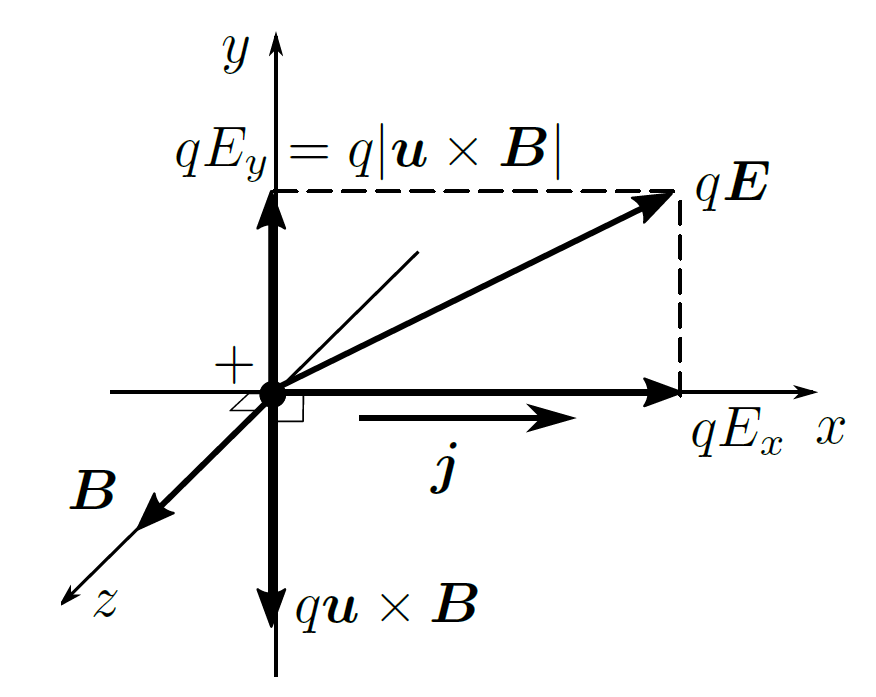
\includegraphics[width=0.46\textwidth]{Teor}
\caption{Силы, действующие на положительный носитель заряда в проводящей
среде при наличии магнитного поля} \label{силы}
\end{center}
\end{figure}

Пусть система содержит носители только одного типа (например,
электроны, как в большинстве металлов). Рассмотрим случай плоской геометрии: пусть ток течёт вдоль оси $x$, а магнитное поле направлено вдоль оси $x$ (см. рис. \ref{силы}). Магнитное поле действует на движущиеся заряды с силой $F_y=-qu_xB_z$ по оси $y$. Ток сможет
течь строго вдоль оси $x$, если заряды в среде перераспределятся таким
образом, чтобы полностью скомпенсировать магнитную силу, создав в
направлении $y$ электрическое поле:
\begin{equation}
\label{E_y}
E_y=u_xB_z=\dfrac{j_x}{nq}B_z
\end{equation}
называемое \textsf{холловским} (здесь $n$ — концентрация носителей). По оси
$x$ носители будут двигаться так, как если бы магнитного поля не было:
$j_x=\sigma_0 E_x (j_y = j_z = 0)$, где $\sigma_0 = qn\mu$ — удельная проводимость среды в отсутствие $B$.

Для исследования зависимости проводимости среды от магнитного
поля в данной работе используется \textsf{мостик Холла} (рис. \ref{мостик}).
\begin{figure}[h!]
\begin{center}
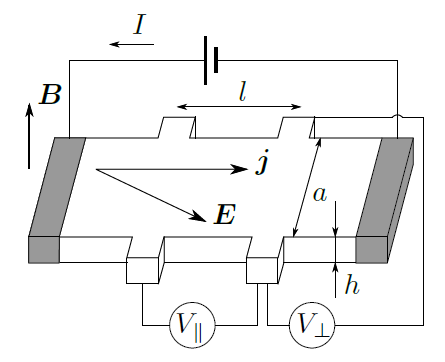
\includegraphics[width=0.46\textwidth]{Мостик}
\caption{Схема для исследования влияния магнитного поля на проводящие
свойства - мостик Холла} \label{мостик}
\end{center}
\end{figure}
В данной схеме ток вынуждают
течь по оси $x$ вдоль плоской пластинки (ширина пластинки $a$, толщина $h$,
длина $l$). Сила Лоренца, действующая со стороны перпендикулярного
пластинке магнитного поля, «прибивает» носители заряда к краям образца,
что создаёт холловское электрическое поле, компенсирующее эту
силу. Поперечное напряжение между краями пластинки (\textsf{холловское 
напряжение}) равно $U_\perp = E_ya$, где, согласно уравнению (\ref{E_y}):
\begin{equation}
E_y=u_xB_z=\dfrac{j_x}{nq}B
\end{equation}
Плотность тока, текущего через образец, равна $j_x=I/ah$, где $I$ — полный
ток, $ah$ — поперечное сечение. Таким образом, для холловского напряжения
имеем
\begin{equation}
\label{формула}
U_\perp = \frac{B}{nqh}\cdot I=R_H\cdot \frac{B}{h}\cdot I,
\end{equation}
где константу
\begin{equation}
R_H = \frac{1}{nq}
\end{equation}
называют \textsf{постоянной Холла}. Знак постоянной Холла определяется
знаком заряда носителей.
Продольная напряжённость электрического поля равна
\begin{equation}
E_x=j_x/\sigma_0
\end{equation}
и падение напряжения $U_\parallel = E_x l$ вдоль пластинки определяется омическим
сопротивлением образца $R_0 = l/(\sigma_0 a h)$:
\begin{equation}
U_\parallel = IR_0
\end{equation}
 


\section{Автоматизация}

\subsection*{Методика существующей работы}
Схема представлена на рис. \ref{старая}. 
Работа состояла из 4 частей: 

Калибровка электромагнита: здесь определяется зависимость магнитной индукции в зазоре электромагнита от тока через магнит. 

Измерение ЭДС Холла – определяется разность потенциалов на образце при различных значениях силы тока через электромагнит и образец. 

Определение знака носителей – делаются выводы о характере проводимости по направлениям тока. 

Измерение удельной проводимости – на образец подается небольшое напряжение, измеряется ток через него.
\begin{figure}[h!]
\begin{center}
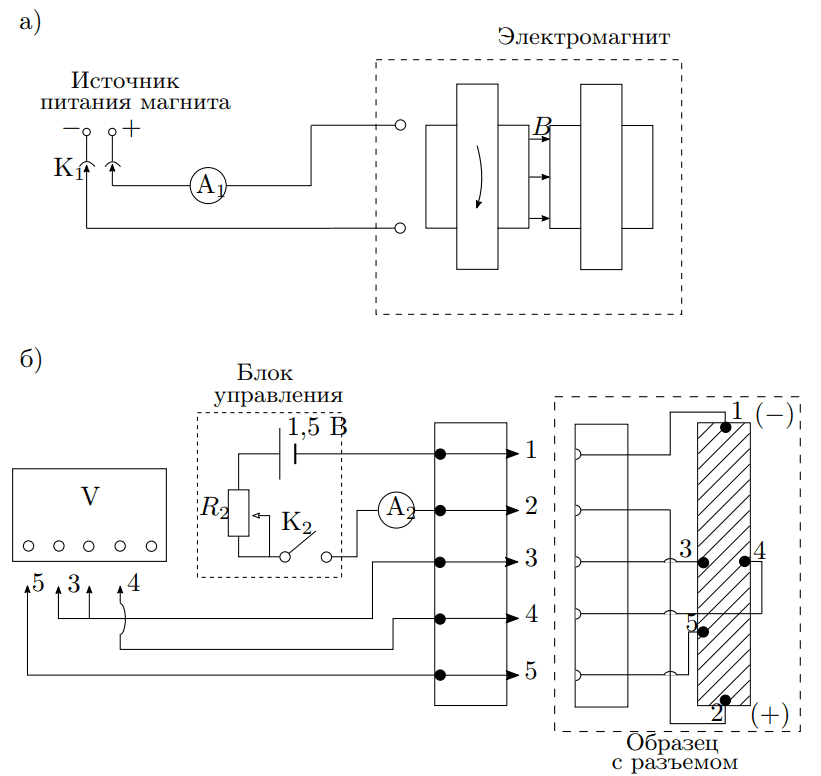
\includegraphics[width=0.66\textwidth]{Схема_ст}
\caption{Схема лабораторной работы для исследования эффекта Холла} \label{старая}
\end{center}
\end{figure}


\subsection*{Проблемы у существующей работы}
У данной работы есть недостатки, основные содержатся в первых двух частях работы. 

\textbf{Градуировка электромагнита}. Каждое измерение необходимо записать в лабораторный журнал. Это достаточно трудоемко, поэтому получается малое количество. Из-за этого у градуировочных коэффициентов возникают высокие погрешности. 

\textbf{Измерение ЭДС Холла}. Измерение тока через образец реализовано с помощью аналогового амперметра с высокой погрешностью. Также невозможно регулировать изменение тока через образец, так как осуществляется при помощи реостата без шкалы. И опять же малое количество измерений из-за высокой трудоемкости.



\subsection*{Обновленный вариант}
Схема обновленной работы представлена на рис. \ref{новая}. Изменения на схемы выделены цветом: все, возможные для подключения, приборы соединены с компьютером. Связь с ними осуществляется при помощи USB-портов. Данные с приборов сохраняются в файлы. Каждая из частей лабораторной представлена в виде отдельного окна в программном обеспечении. Добавлена часть с автоматическим построением графиков и вычислением постоянных образца. Заменены некоторые приборы: аналоговый амперметр на цифровой, батарейка с реостатом без шкалы на программируемый источник питания.

\begin{figure}[h!]
\begin{center}
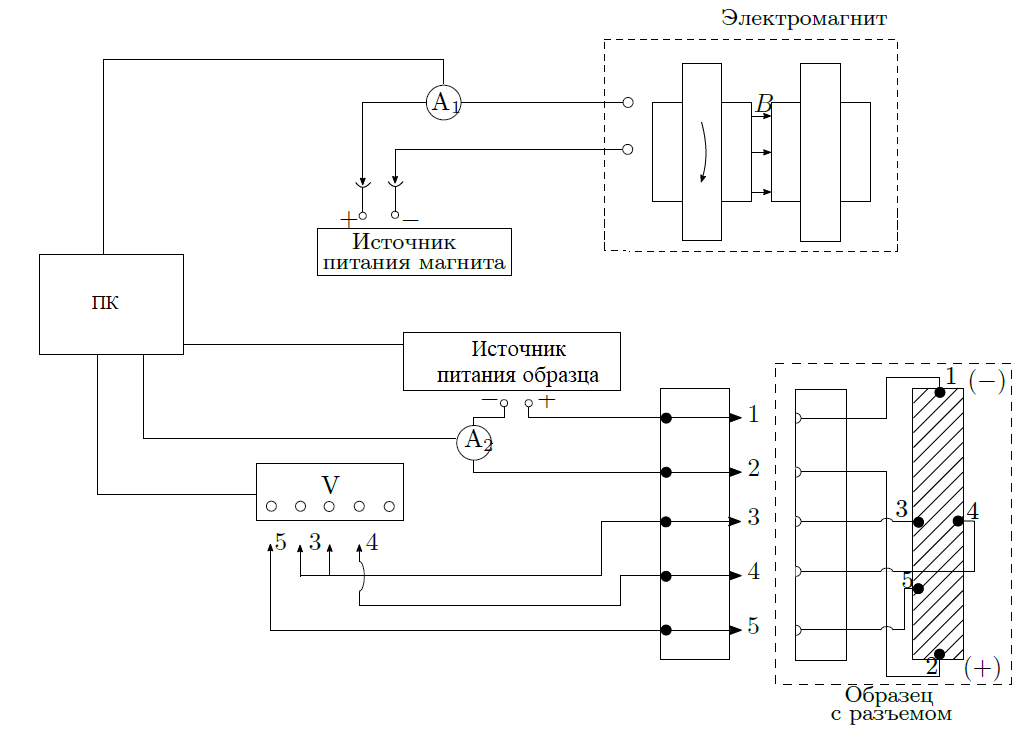
\includegraphics[width=0.76\textwidth]{Установка}
\caption{Обновленная схема лабораторной работы для исследования эффекта Холла} \label{новая}
\end{center}
\end{figure}

Кроме схемы установки изменения видны и на фотографиях (рис. \ref{старое_фото}, \ref{новое_фото}).


\begin{figure}[h!]
\begin{center}
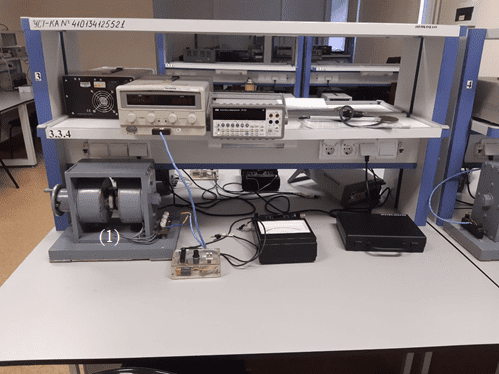
\includegraphics[width=0.85\textwidth]{старая_картинка}
\caption{Фотография установки по исследованию эффекта Холла, исходный вариант)} \label{старое_фото}
\end{center}
\end{figure}

\begin{figure}[h!]
\begin{center}
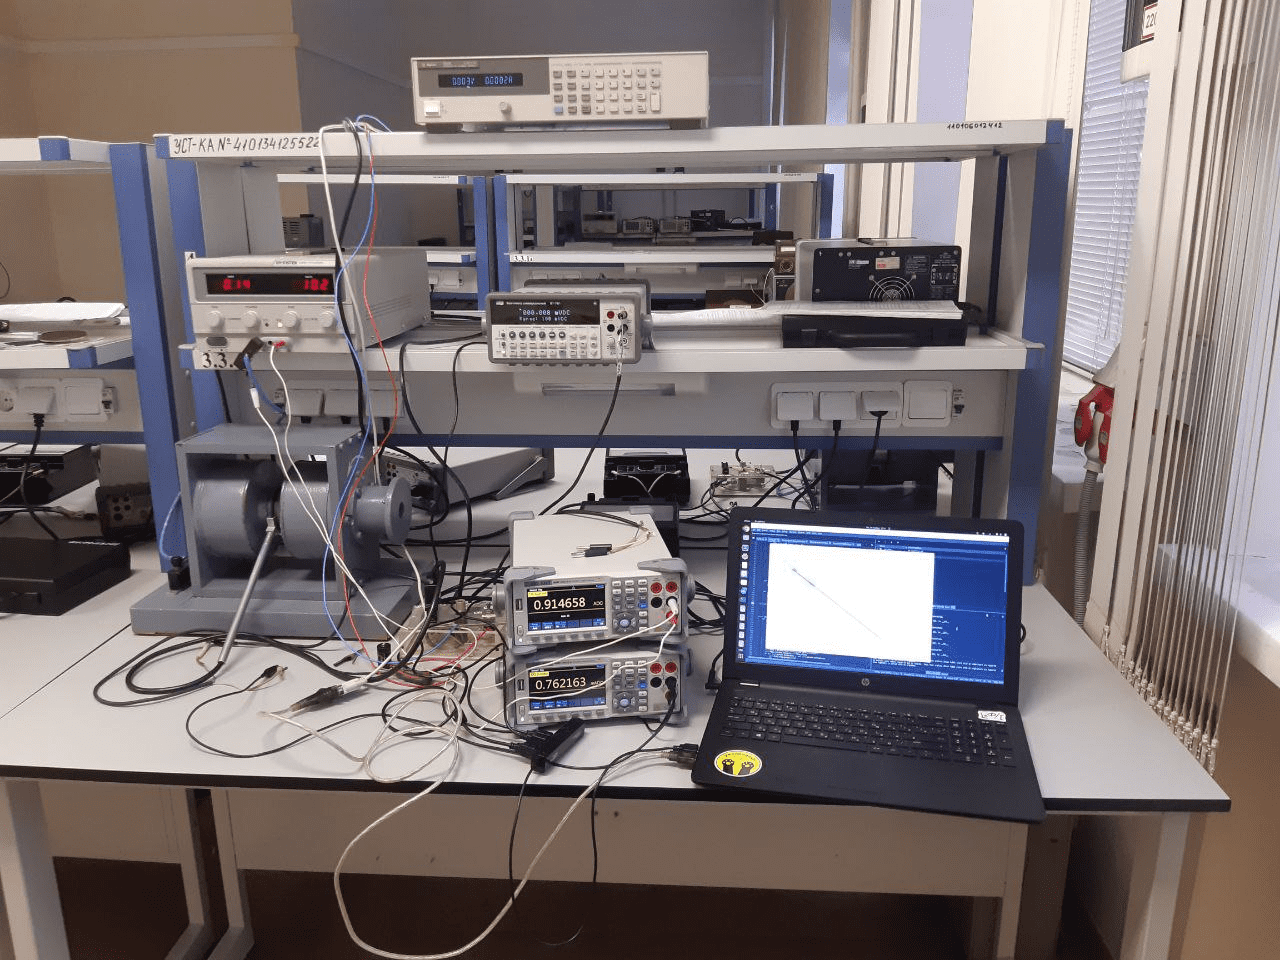
\includegraphics[width=0.85\textwidth]{новая_картинка}
\caption{Фотография установки по исследованию эффекта Холла, обновленный вариант)} \label{новое_фото}
\end{center}
\end{figure}


У обновленного варианта есть свои преимущества: 

1) Автоматическое получение данных понижает трудоемкость измерений и позволяет сделать большее их число. Из-за этого повышается точность постоянных образца. 

2) Также аналоговый амперметр заменен более точным цифровым и добавлен источник питания образца с возможность регулировки тока. 

3) Есть автоматический контроль чрезмерно больших токов через образец, что предотвращает его повреждение. 

4) Появилась возможность сделать выводы о работе сразу из-за компьютерной обработки результатов.



\subsection*{Результаты автоматизации}
Лабораторная работа была выполнена на исходной установке и на автоматизированной. Результаты в виде зависимости ЭДС Холла от тока через образец представлены на рис. \ref{старый_график} и рис. \ref{новый_график}. 
Изменения заметны. Во-первых, количество точек значительно выросло: с 50 до 200, то есть в 4 раза. Во-вторых, погрешности отдельных точек уменьшились: только за счет смены амперметра в 300 раз. В-третьих, погрешность коэффицента наклона прямой уменьшилась в более чем 3 раза (с 11 \% до 3).

\begin{figure}[h!]
\begin{center}
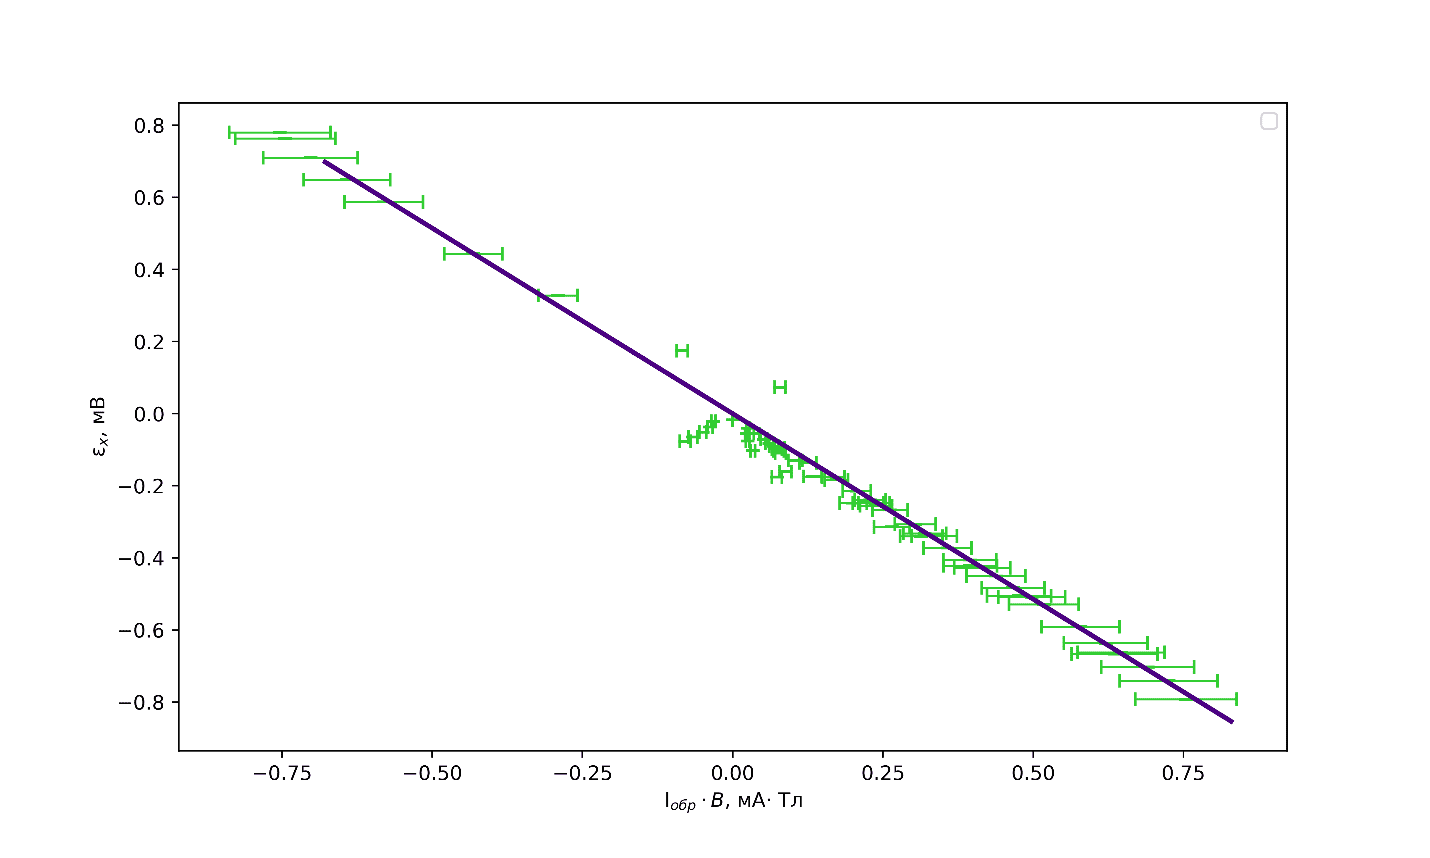
\includegraphics[width=0.86\textwidth]{Старая}
\caption{Зависимость ЭДС Холла от тока через образец и магнитной индукции в исходном варианте работы} \label{старый_график}
\end{center}
\end{figure}

\begin{figure}[h!]
\begin{center}
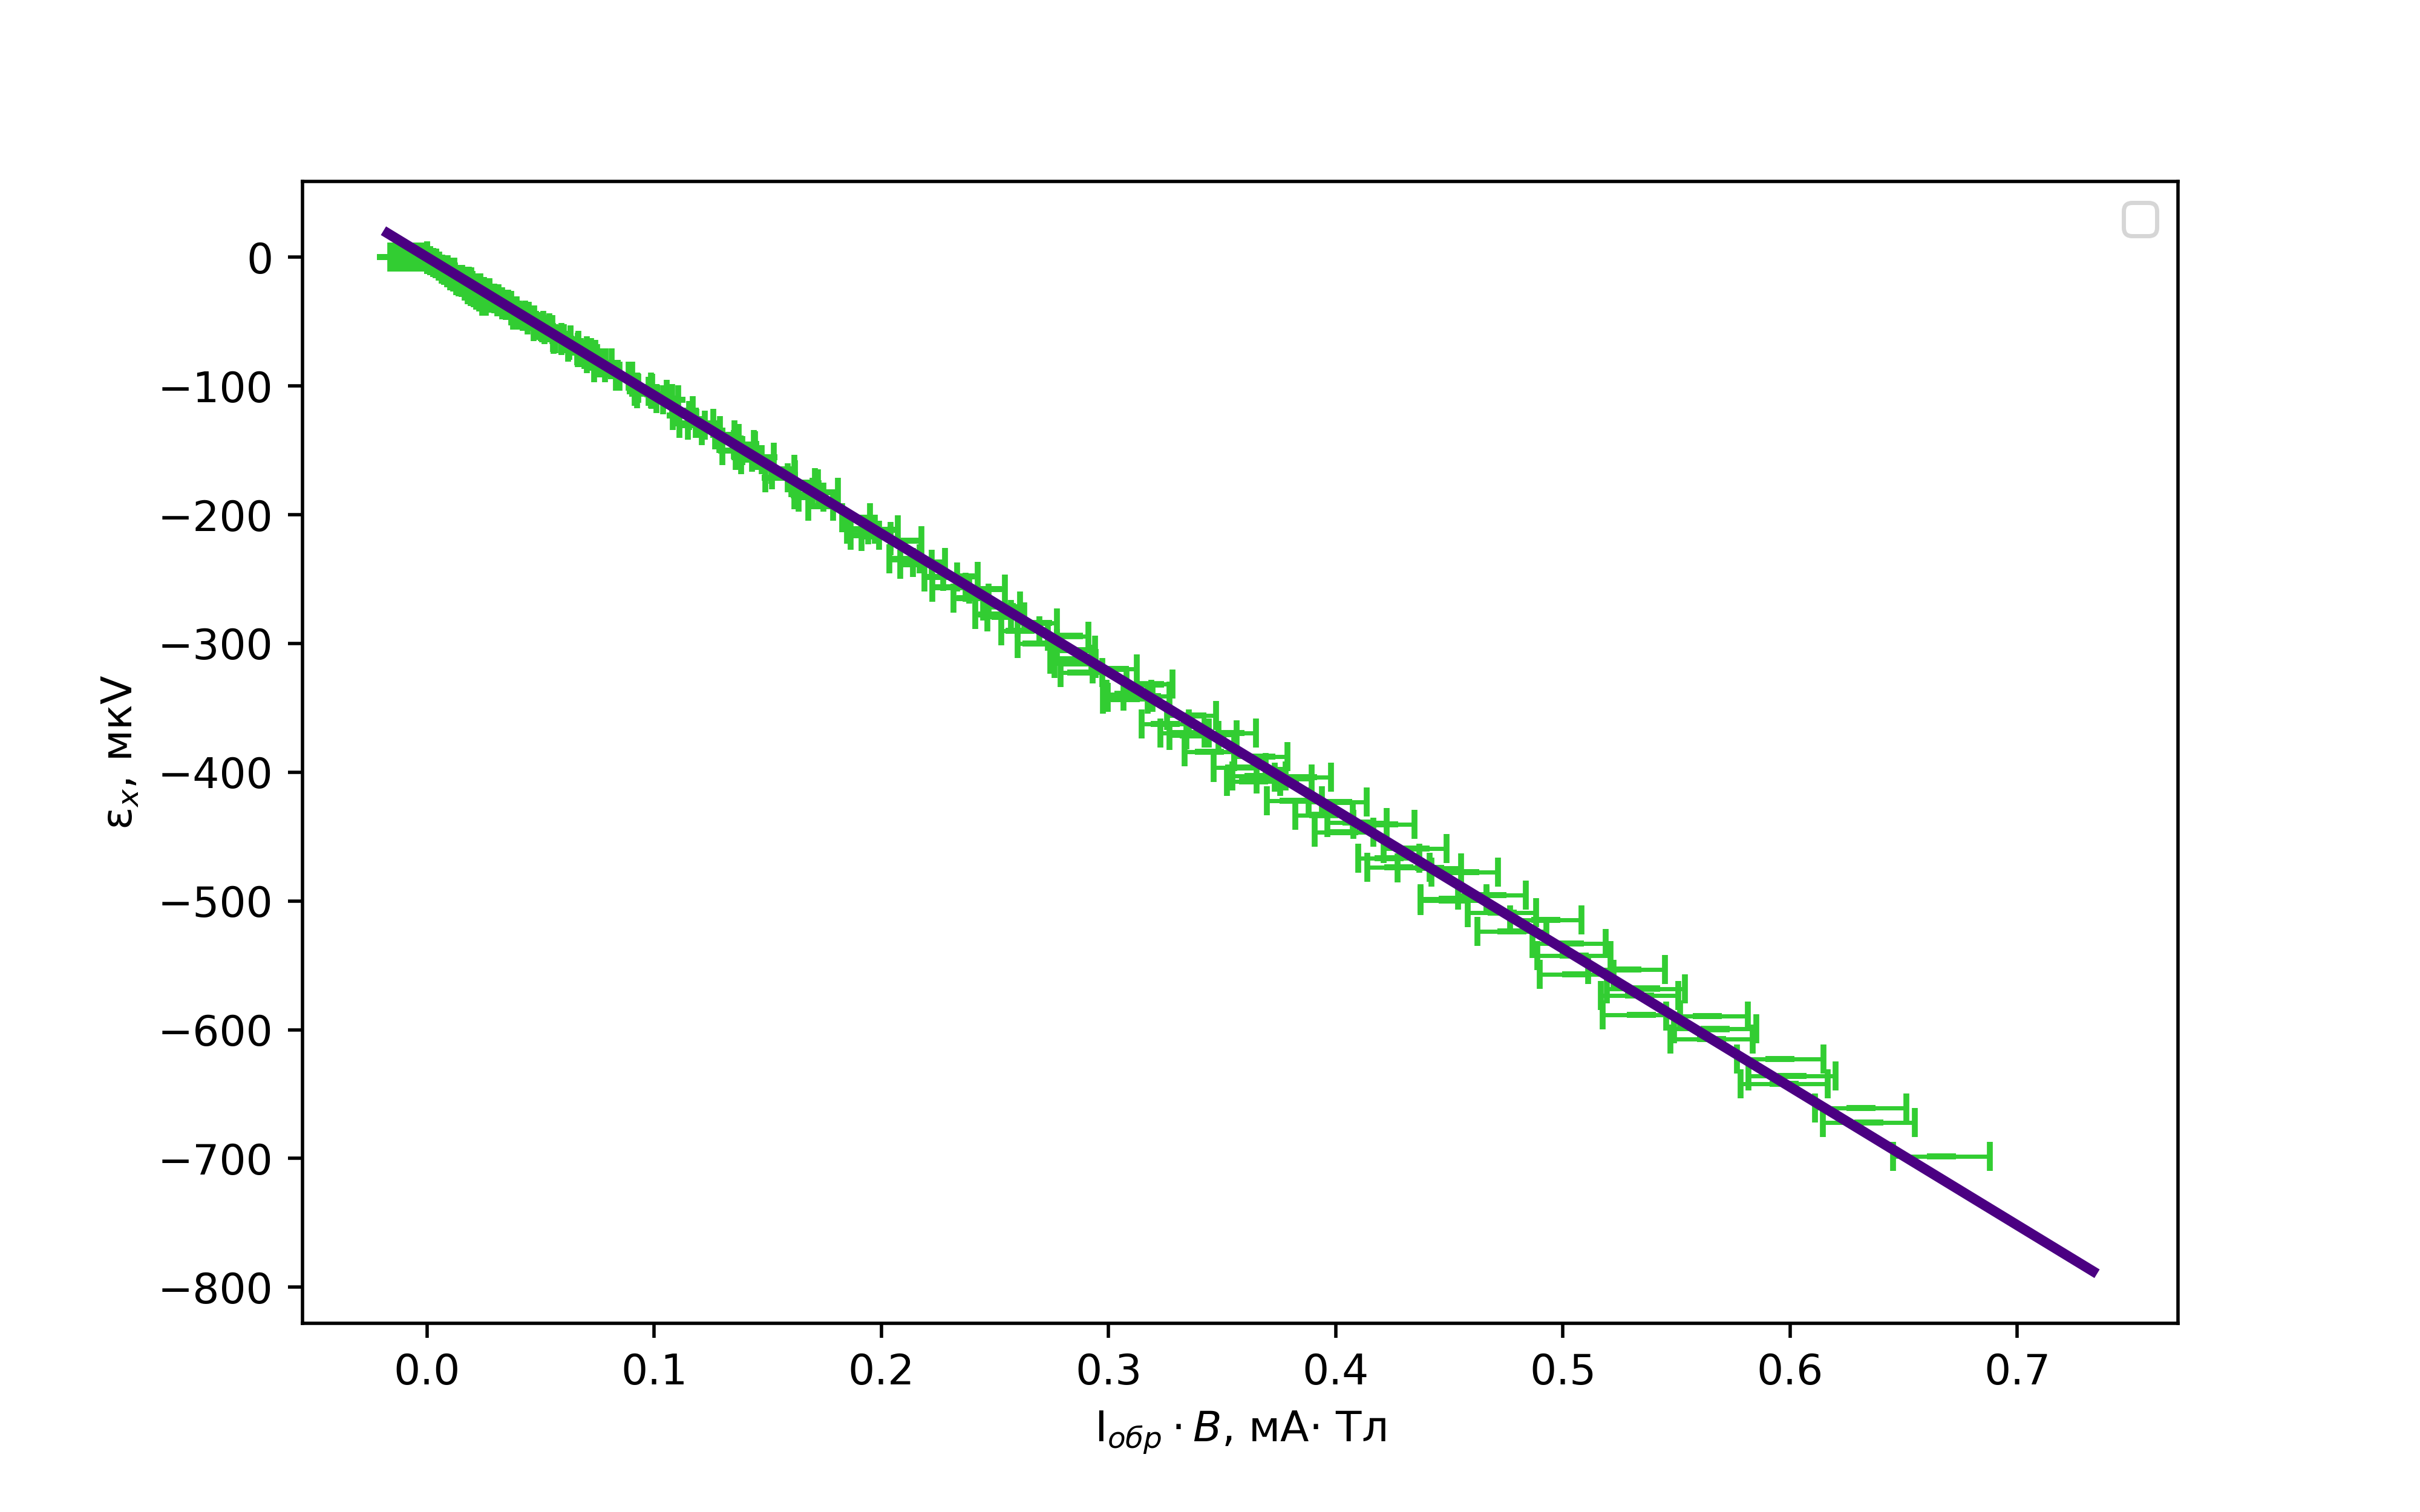
\includegraphics[width=0.78\textwidth]{Chart}
\caption{Зависимость ЭДС Холла от тока через образец и магнитной индукции в обновленном варианте работы} \label{новый_график}
\end{center}
\end{figure}

\subsection*{Новое качество}
Однако в процессе измерений было обнаружено, что зависимость магнитного поля в электромагните от тока через него не линейна (рис. \ref{grad}).

\begin{figure}[h!]
\begin{center}
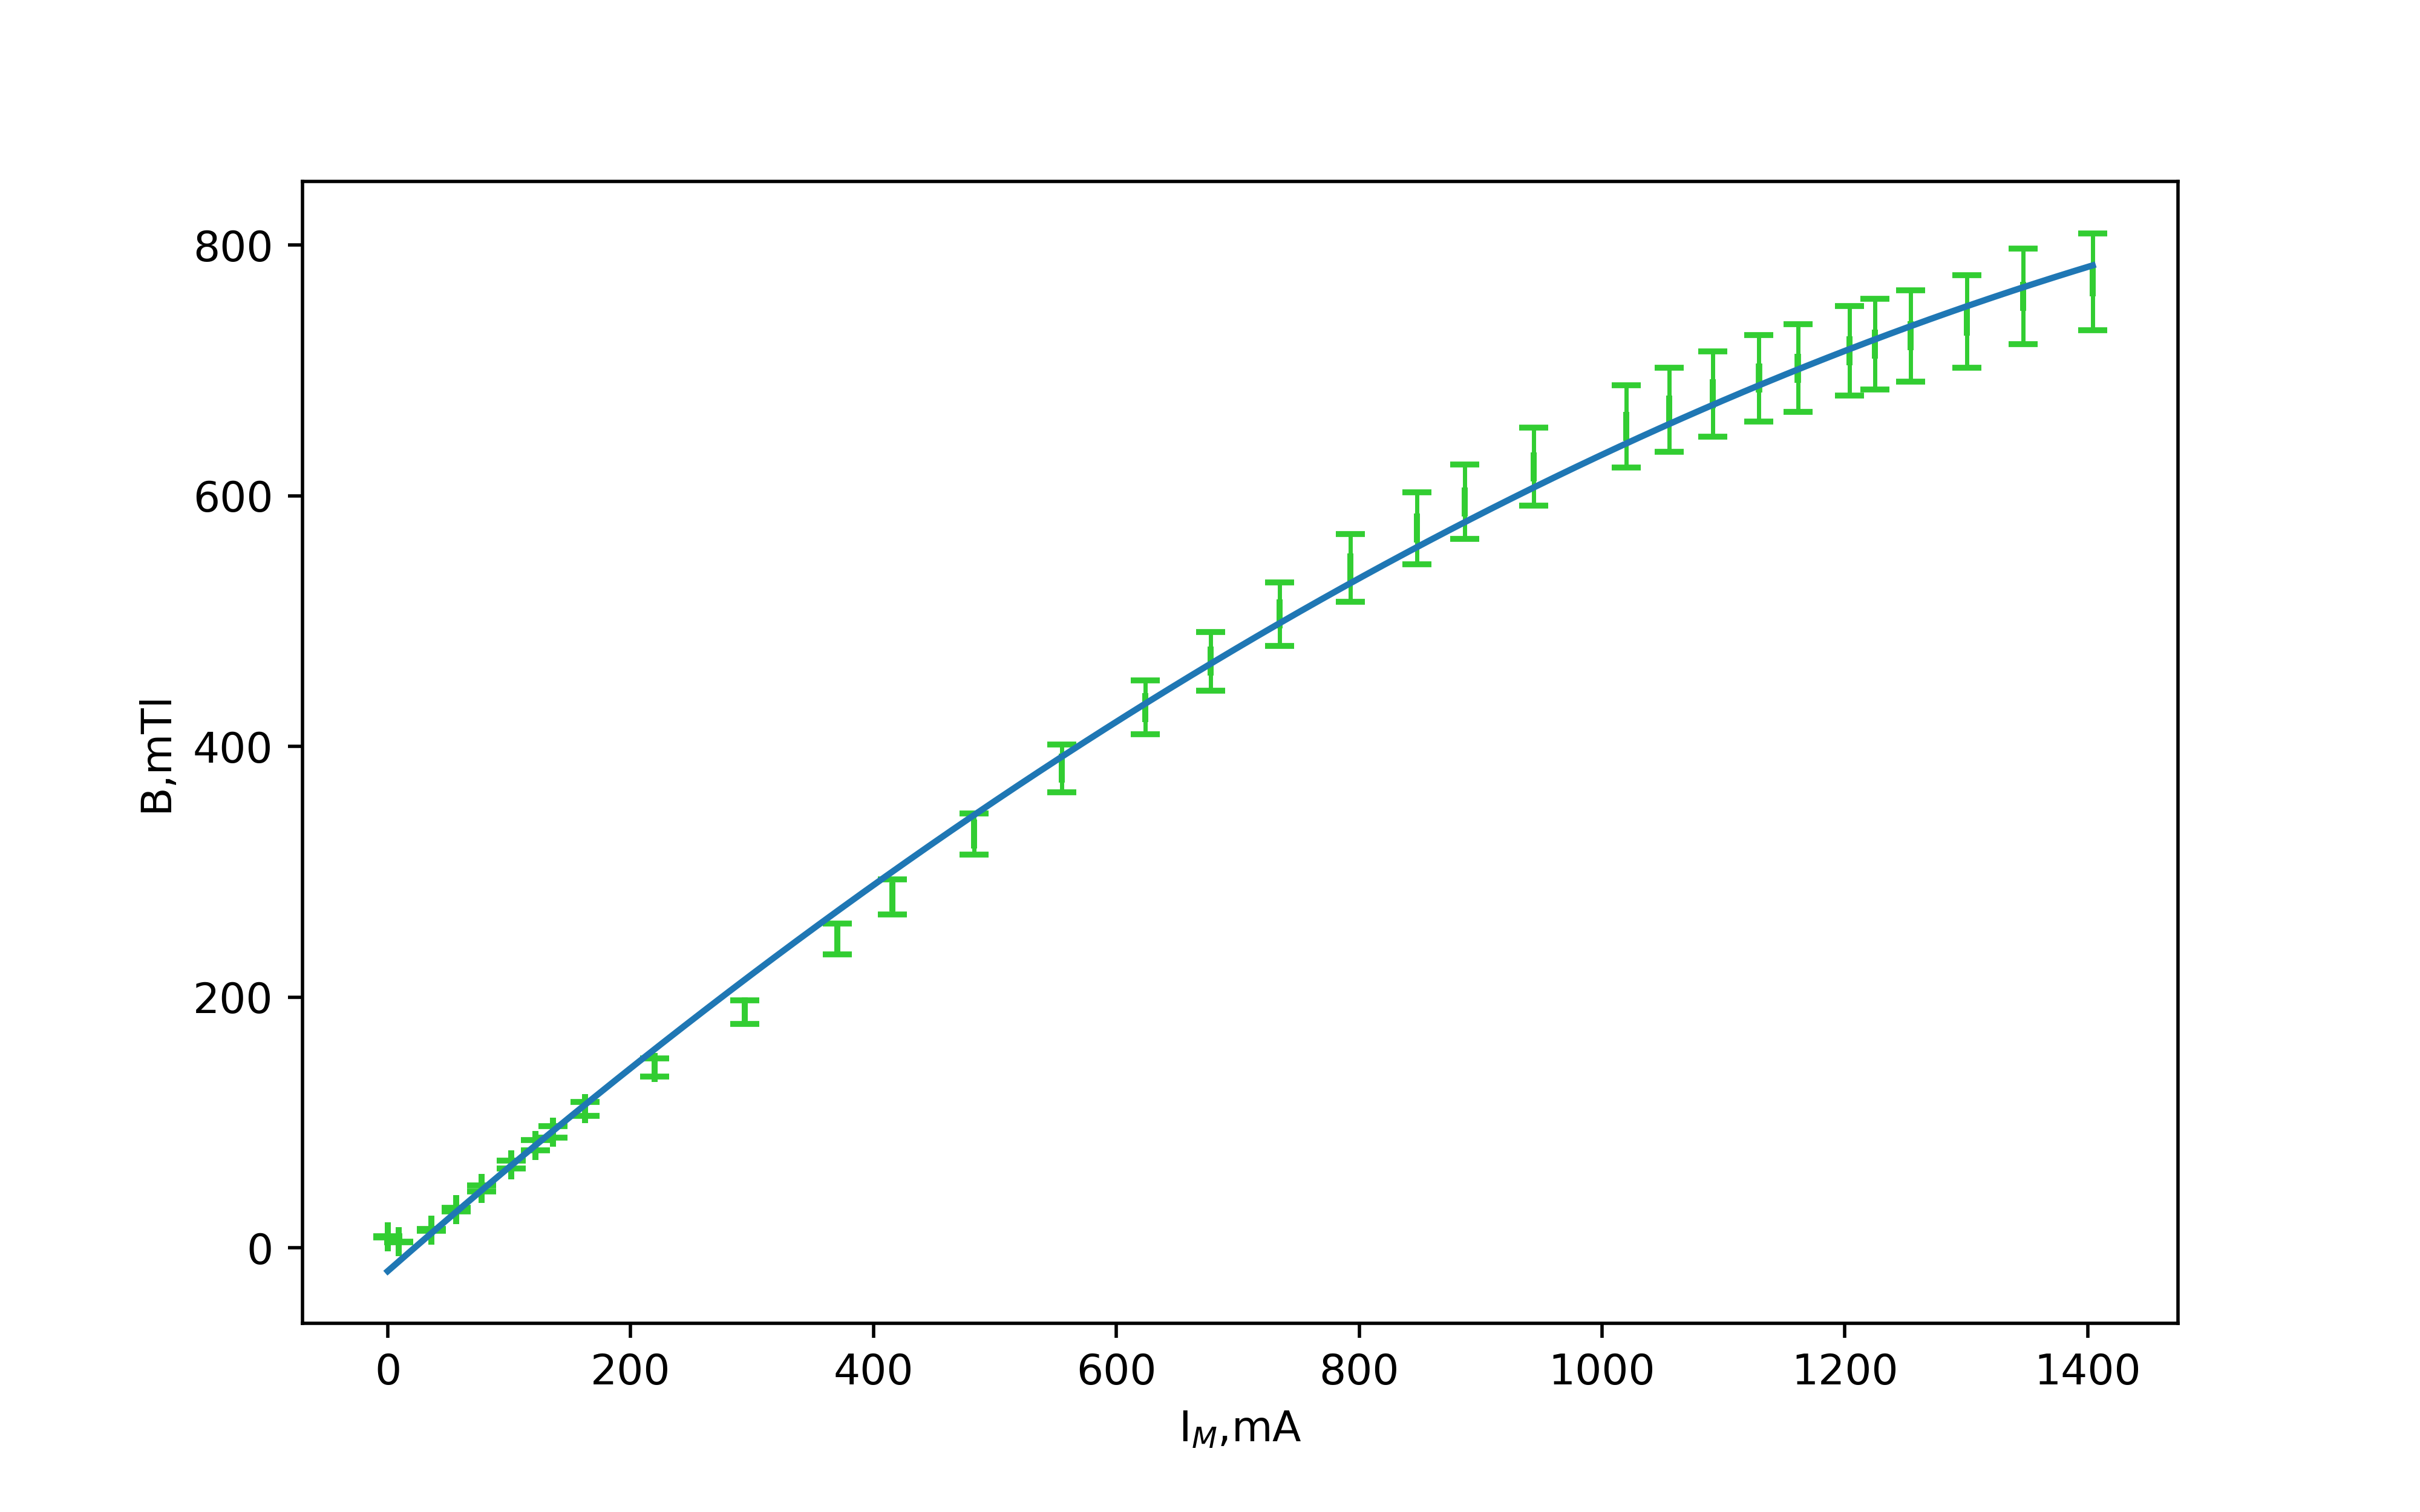
\includegraphics[width=0.78\textwidth]{Graduation_chart}
\caption{Зависимость магнитной индукции в зазоре электромагнита от тока через него} \label{grad}
\end{center}
\end{figure}
Но из теоремы о циркуляции магнитного поля (в системе СГС): 
\begin{equation}
\oint_L H \cdot dl =\frac{4\pi}{c}J
\end{equation}
Видно, что ток и напряженность магнитного поля связаны прямой пропорциональностью. То есть есть нелинейная зависимость $B$ от $H$ в электромагните. 

Существуют вещества трех типов: пара-, диа- и ферромагнетики. Однако для первых двух зависимость $B$ от $H$ линейна. Из чего следует, что электромагнит создан из ферромагнитного материала (таковым является, например, железо). 

Теперь интересно сравнить полученную зависимость с теоретической ( в форме графика на рис. \ref{фер}. Они, как и ожидалось, подобны друг другу, что подтверждает материал электромагнита. 

\begin{figure}[h!]
\begin{center}
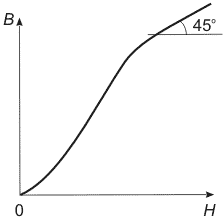
\includegraphics[width=0.38\textwidth]{ферро}
\caption{Теоретическая зависимость магнитной индукции от напряженности магнитного поля для ферромагнетика} \label{фер}
\end{center}
\end{figure}


\section{Проблемы}
\subsection*{Неавтоматизированные части}
На текущий момент работа не является полностью автоматизированной. Это не получилось в данном семестре, так как не было высоковольтного источника питания и измерителя магнитной индукции с возможностью программирования. Еще есть проблема с подключением в виде коробки (рис. \ref{коробка}). Но изменить ее было невозможным, так как установку каждый раз необходимо было возвращать в исходное состояние. 

\begin{figure}[h!]
\begin{center}
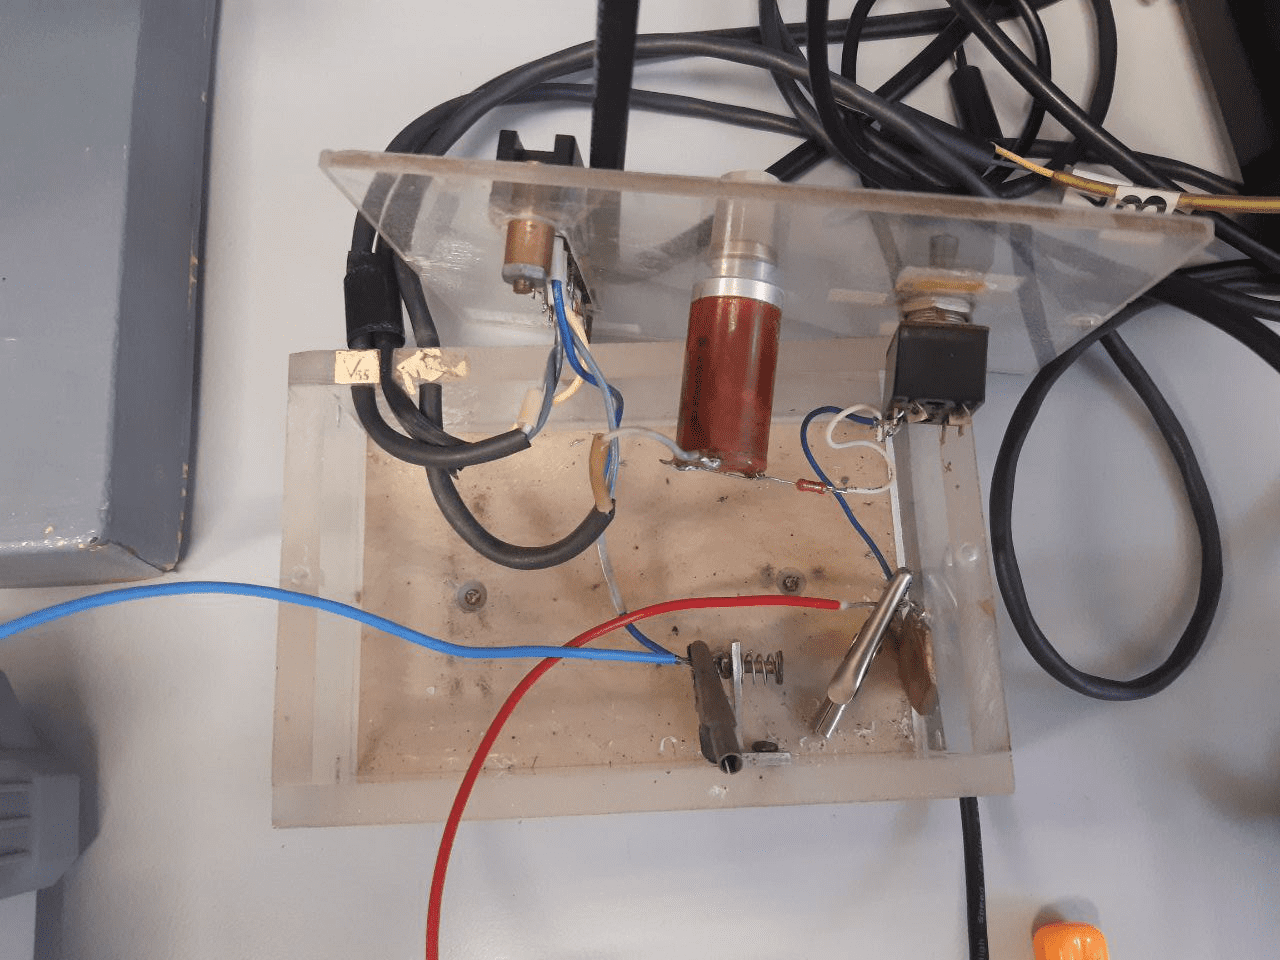
\includegraphics[width=0.68\textwidth]{corob}
\caption{Блок управления лабораторной работой} \label{коробка}
\end{center}
\end{figure}

\subsection*{Неудавшиеся измерения}
Были предприняты попытки обнаружить эффект Холла в металлах, использую то же оборудование. Однако в металлах постоянная Холла $R_H \approx 10^{-10}$, толщина образца порядка сотых долей миллиметра, пропускаемый допустимый ток около 1 мА, магнитная индукция около 1 Тл. Поэтому (из формулы \ref{формула}) измеряемое напряжение было бы порядка $10^{-9}$ В, предел вольтметра при этом - десятые доли мкВ. Поэтому измерения не привели ни к чему хорошему.


\section{Выводы}

\hspace{5mm} 1. Получение данных напрямую с приборов  увеличило скорость работы

2. Автоматизация и замена аналоговых приборов сделали работу существенно точнее

3. Благодаря автоматизации удалось достаточно быстро получить зависимость магнитной индукции от тока в электромагните, сделать вывод о ферромагнетизме материала.

4. Однако есть и проблемы, но их решение существует.


\end{document}